\section{Wat zijn zelflerende computersystemen?}

\subsection{Inleiding}
Elk jaar boekt de mens grootschalige vorderingen op het gebied van computers, zowel hardware als software. Iets waar wij echter nog niet in geslaagd zijn te maken is een ware \textbf{ Artificial Intelligence}, al lukt het steeds beter de schijn van denken te creëren. Voorbeelden zijn de \textit{persoonlijke assistenten} die inmiddels in elke smartphone geïntegreerd zijn. \textit{Siri}, \textit{Google Now} en \textit{Coratana} maken gebruik van spraakherkenning om de gebruiker de gevraagde informatie te tonen, maar denken zoals mensen doen ze hierbij niet. Hoe een computersysteem toch beter kan worden in het imiteren van menselijk gedrag en van zijn eigen fouten kan leren onderzoeken in deze deelvraag.


\subsection{Verschillende algoritmes}
Computers hebben geen dus bewustzijn. Om deze reden kunnen ze niet zelf bepalen iets te doen. Waar computers wel in uitblinken, is het uitvoeren van taken die ze zijn opgelegd. Vaak komen deze taken in de vorm van code. Via code kan je computers opdrachten geven, bijvoorbeeld laat een scherm zien. De boodschap valt echter niet op deze manier over te brengen, afhankelijk van de taal waarin je programmeert zijn er vaste commando’s waar de computer op zal reageren.
Naarmate de opdracht die je een computer wil laten uitvoeren complexer worden, zal ook het gebruik in deze commando’s een verandering zien. Hier komen algoritmes in het spel. Een algoritme is een soort stappenplan voor de computer, waarin een complexere handeling in duidelijke opdrachten weergegeven wordt. De volgende definitie geeft een betekenis in de meest algemene zin: een algoritme is een eindige reeks instructies om vanaf een beginpunt een bepaald doel te bereiken.\cite{WoordenOrg}

Een toegankelijke vergelijking is koken. Er is een \textbf{input} van voedsel waar uiteindelijk een gerecht uit moet komen, de \textbf{output}. Voor het tot stand komen van dit gerecht gebruik je misschien een recept. Dit recept is als het ware het algoritme.
Uit de gegeven definitie kan is af te leiden dat het aantal mogelijke algoritmes ontzettend groot is. Niet alleen is het een ruim begrip, ook kan het desbetreffende doel waarschijnlijk op meerdere manieren bereikt worden. In deze verschillende methodes kan de een echter beter zijn dan de andere, bijvoorbeeld door efficiënter te zijn.

Uiteraard zijn er ook vele algoritmes die gebruik maken van toepassingen, zoals een \textbf{queue} en een \textbf{stack}, die betrekking hebben tot ons onderwerp. Enkele hiervan zullen hier beschreven worden:

\subsection{Breadth-first search (BFS)}

\subsection{Depth-first search (DFS)}

\subsection{Voorbeelden algoritmes}

\subsubsection{Breadth-first search}

\subsubsection{Depth-first search}

\subsection{Zelflerend?}
Breadth-first search en Depth-first search zijn beide algoritmes met vele toepassingen. Toch kunnen beide algoritmes niet als zelflerend worden beschouwd, ze verbeteren hun manier van zoeken namelijk niet. Hoe zit een zelflerend systeem dan wel in elkaar? Hoe kan een algoritme zichzelf verbeteren?

\subsection{Machine learning}
Een zelflerend systeem is een algoritme gebaseerd op machine learning. Machine learning werd door Arthur Samuel, een pionier op dit gebied, gedefinieerd als: 
\textit{A field of study that gives computers the ability to learn without being explicitly programmed.} \cite{ArthurSamuel} 
In tegenstelling tot de eerder genoemde algoritmes is een zelflerend systeem in staat zichzelf te verbeteren. Hierdoor kan het taken uitvoeren waarbij reguliere algoritmes tekort schieten. Welke taken dit betreft, zullen we in de derde deelvraag behandelen. 

\begin{figure}[h]
  \centering
    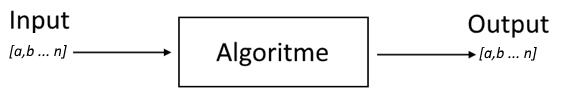
\includegraphics[width=\textwidth]{algorithm1.png}
  \caption{Schematische weergave van een zelflerend systeem}
  \label{fig:algorithm1}
\end{figure}

In figuur \ref{fig:algorithm1}  is een schematische weergave van een zelflerend systeem afgebeeld. Bepaalde input data gaat het systeem in en bepaalde output data komt het systeem uit. De input en output data bestaat uit \'e\'en of meerdere getallen. Als de input simpelweg een reeks getallen betreft, zal dit direct als input gebruikt kunnen worden. In het geval dat de input uit een ander datatype bestaat, zoals een plaatje, zal dit omgezet moeten worden in een reeks getallen voordat het in een zelflerend systeem gebruikt kan worden. Het algoritme zal deze getallen bewerken tot de gewenste output. Deze output wordt eveneens in getallen gegeven. Waar nodig zullen deze getallen dus weer moeten worden omgezet tot het gewenste datatype.

Er zijn veel verschillende algoritmes die gebruikt kunnen worden voor een zelflerend systeem. Elk algoritme heeft voor- en nadelen en is geschikt voor andere doeleinden. Een aantal van deze algoritmes zullen we in de tweede deelvraag behandelen. 

\subsection{Training}

Een zelflerend systeem begint in de meeste gevallen zonder enige kennis van de data. Om de gewenste output te kunnen produceren is het dus nodig om het systeem eerst input data te geven zodat het kan leren. Dit proces wordt het \textbf{trainen} genoemd. Voor het trainen van een zelflerend systeem is training data nodig. Deze data moet gelijk of gelijkwaardig zijn aan de \textit{echte} data. De training data kan in veel verschillende vormen voorkomen en de manier van trainen is afhankelijk van de vorm van de (training) data. In figuur \ref{fig:algorithm2}  is te zien dat het trainen los staat van het algoritme. Dit verschil zullen we in de volgende deelvraag wat duidelijker maken. 
Er zijn drie prominente manieren waarop een zelflerend systeem getraind kan worden: \textbf{supervised}, \textbf{unsupervised} en \textbf{reinforcement learning}.

\begin{figure}[h]
  \centering
    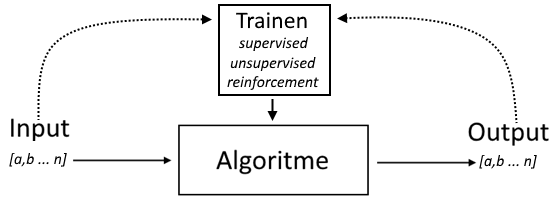
\includegraphics[width=\textwidth]{algorithm2.png}
  \caption{Schematische weergave van een zelflerend systeem}
  \label{fig:algorithm2}
\end{figure}

\subsubsection{Supervised Learning}
In het geval van supervised learning heb je te maken met \textbf{labeled} training data. Anders gezegd: van een bepaalde input is de gewenste output al bekend. Een klassiek voorbeeld van een labeled dataset is een dataset van huisprijzen en huiseigenschappen (zie figuur \ref{fig:LabeledDataset})

\begin{table}[h]
\centering
\begin{tabular}{llll}
\hline
\multicolumn{1}{c}{\multirow{2}{*}{Huisprijs (output)}} & \multicolumn{3}{c}{Huiseigenschappen (input)} \\
\multicolumn{1}{c}{} & \multicolumn{1}{c}{Woonoppervlakte} & \multicolumn{1}{c}{Perceeloppervlakte} & \multicolumn{1}{c}{Aantal Kamers} \\ \hline
€ 519.000 & 124 m² & 311 m² & 4 \\
€ 569.000 & 133 m² & 309 m² & 5 \\
€ 569.500 & 170 m² & 310 m² & 6 \\ \hline
\end{tabular}
\caption{Labeled dataset Bron: http://www.funda.nl/koop/huizen/ }
\label{fig:LabeledDataset}
\end{table}
Bij de training dataset van figuur \ref{fig:LabeledDataset} is de gegeven input de huiseigenschappen en de gewenste output de huisprijs. Het systeem wordt met deze dataset getraind. Hierdoor leert het een output te produceren die steeds dichter bij de gewenste output ligt. Als er een verband bestaat tussen de huiseigenschappen en de huisprijs, wat waarschijnlijk het geval is, zal het zelflerende systeem na genoeg trainen in staat zijn zelf bij nieuwe huiseigenschappen een huisprijs te voorspellen. \cite{MLCourse1}


\subsubsection{Unsupervised Learning}
Unsupervised learning kan gebruikt worden bij een \textbf{unlabeled} dataset ofwel, een dataset waarbij de data niet geclassificeerd is en er geen gewenste output bekend is. Als je een dataset hebt van heel veel niet-geordende foto’s is het niet mogelijk om dit te classificeren. Als een deel van de dataset gelabeld wordt, zal met behulp van supervised learning de rest van de dataset geclassificeerd kunnen worden. Dit is echter in veel gevallen niet mogelijk, bijvoorbeeld doordat de dataset enorm groot is of er zodanig veel verschillende groepen bestaan dat het menselijk niet mogelijk is ook maar een deel te labelen. Ook kan het zo zijn dat men niet weet of er een verband aanwezig is. 
Kortom: unsupervised learning wordt gebruikt voor het classificeren van data, zonder dat er groepen vooraf gedefinieerd zijn. Met behulp van deze vorm van training zullen in een grote dataset verbanden kunnen worden ontdekt, die men misschien niet zonder hulp had kunnen achterhalen.\cite{MLCourse2}

\subsubsection{Reinforcement Learning}
Reinforcement learning is een zeer specifieke soort van leren. Er is bij deze vorm van learning geen dataset met input data, maar is er een bepaalde \textbf{context}. In deze context bevindt zich een \textbf{agent}. Een agent is een object dat bepaalde opdrachten kan uitvoeren. De context is een wereld waarin deze agent zich bevindt. Door de agent bij bepaalde acties pluspunten of minpunten te geven kun je bepaald gedrag bevorderen.  

\begin{figure}[h]
  \centering
    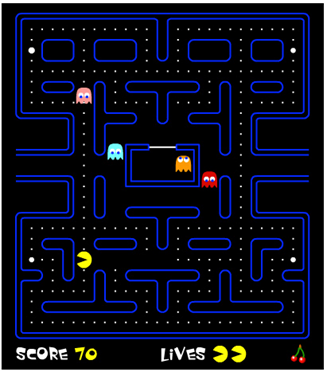
\includegraphics[width=0.5\textwidth]{pacman.png}
  \caption{Pacman}
  \label{fig:Pacman}
\end{figure}

In figuur \ref{fig:Pacman} is het spel pacman te zien. De agent is hierbij pacman, deze kan namelijk een object dat bepaalde opdrachten kan uitvoeren zoals: loop naar links, loop naar rechts. De context is hierbij het level, ofwel: de positie van de muren (de blauwe obstakels), de posities van de \textit{ghosts} (de geleurde vijanden), de posities van de \textit{pac-dots} (de kleine stipjes, ofwel punten) en de posities van de\textit{power-pellets} (de grotere stipjes). \cite{PacWiki} Het eten van de pac-dots is positief, het geraakt worden door de ghosts is negatief. Door reinforcement learing toe te passen op het spel zal de agent steeds beter worden in het spelen van het spel. 

\subsection{Conclusie}
Zelflerende computersystemen zijn algoritmes gebaseerd op machine learning. Een zelflerend systeem verschilt van reguliere algoritmes zoals breadth-first search en depth-first search doordat ze in staat zijn zichzelf te verbeteren

\bibliography{references}
\bibliographystyle{plain}